\documentclass[11pt,aspectratio=1610,xcolor=dvipsnames]{beamer}

\usetheme[
    background=light,
    numbering=fraction,
    block=fill,
    progressbar=frametitle
]{metropolis}

\graphicspath{{img/}}

\usepackage[style=authortitle-ibid,backend=biber]{biblatex}
\addbibresource{refs.bib}
\setbeamerfont{footnote}{size=\scriptsize}

\usepackage{physics}
\usepackage{mathtools}
\usepackage{bbm}
\usepackage{booktabs}
\usepackage[most,skins,theorems]{tcolorbox}
\tcbset{variables/.style={colback=yellow!20,colframe=yellow}}
\usepackage{tikz}
\usetikzlibrary{shapes.geometric, arrows, shadows}
\usetikzlibrary{fit, backgrounds}



% \colorlet{LightLavender}{Lavender!40!}
\newtcolorbox{prob}{colback=red!5!white,colframe=red!75!black}
\usefonttheme[onlymath]{serif}
\usepackage{quantikz}
\usepackage{qrcode}
\usepackage{pgfplots}
\usepackage{pythonhighlight}

\newcommand{\R}{\mathbb{R}}
\newcommand{\U}[1]{\mathsf{U}(#1)}
\newcommand{\defeq}{\stackrel{\text{\tiny def}}{=}}

\titlegraphic{
\includegraphics[width=0.3\textwidth]{unitary_fund_logo.png}}

\title{Hypothesis Testing for Error Mitigation}
\subtitle{Quantum Wednesday}
\date{Mar 8, 2023}
\author{Nate Stemen}


\begin{document}

\maketitle

\begin{frame}{Today's Paper}
	\begin{figure}[h]
		\centering
		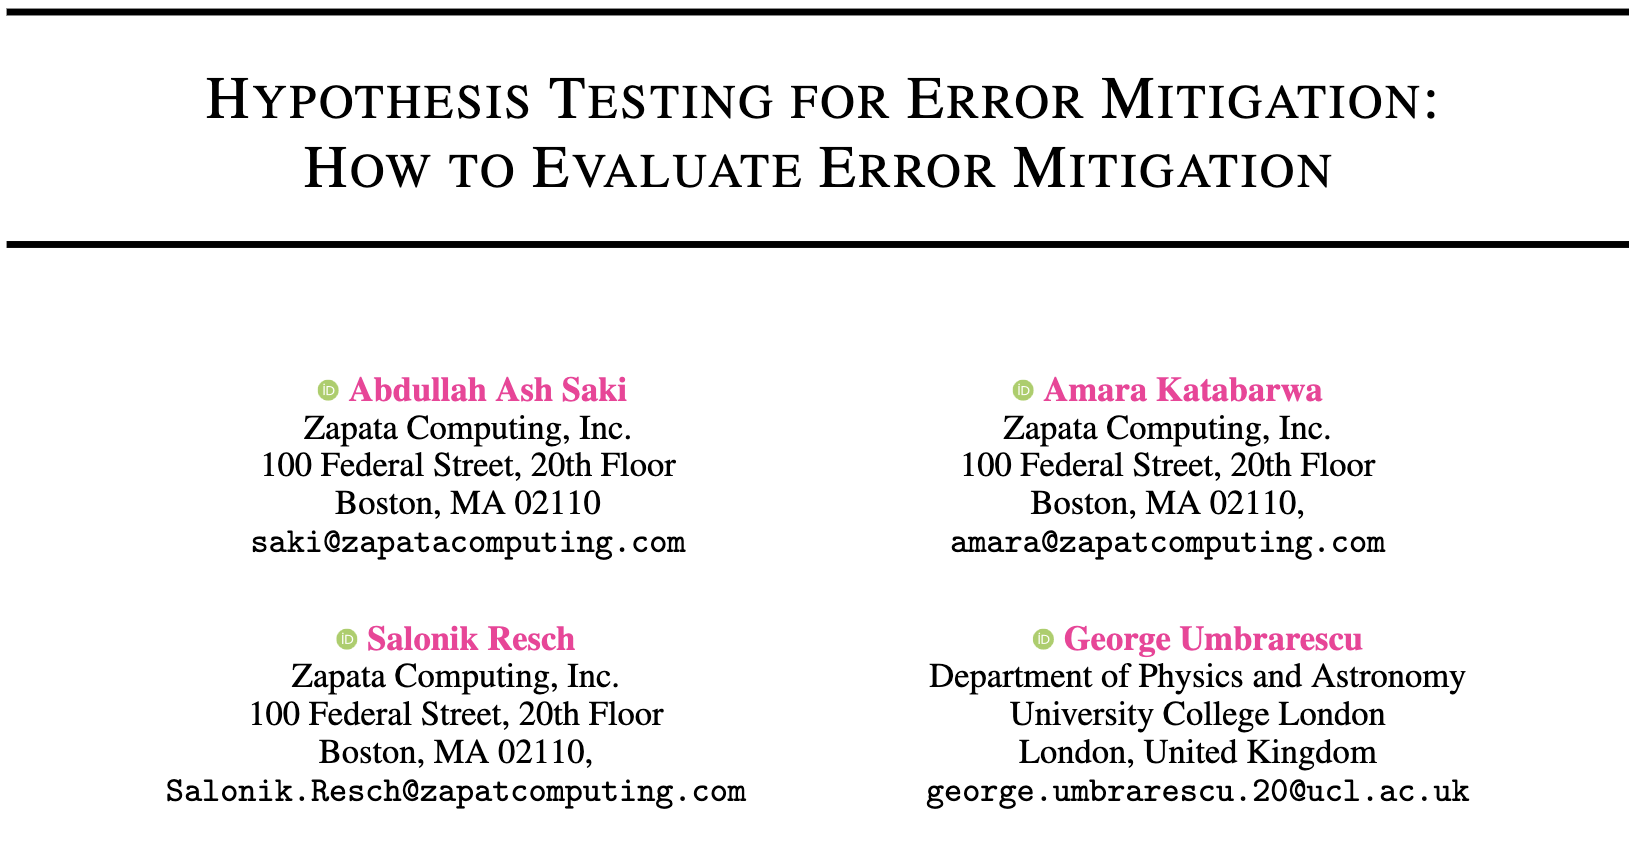
\includegraphics[width=0.8\textwidth]{paper.png}
	\end{figure}
	\begin{center}
		\url{https://arxiv.org/abs/2301.02690}
	\end{center}
\end{frame}

\begin{frame}{Overview}
	\begin{enumerate}
		\item What is hypothesis testing?
		\item How do we compare error mitigation methods?
		\item How do we know what error mitigation techniques are statistically important in a stacked sequence?
		\item Evaluation pipeline
		\item Results
	\end{enumerate}
\end{frame}

\newcommand{\RZ}[1]{\scriptstyle{R_Z(#1)}}
\begin{frame}{Experimental setup}
	\begin{quantikz}[row sep=0.1cm, column sep=0.15cm]
		& \gate{H} & \ctrl{1} & \qw                & \ctrl{1} & \qw      & \qw                & \qw      & \ctrl{2} & \qw                & \ctrl{2} & \qw      & \qw                & \qw      & \ctrl{3} & \qw                & \ctrl{3} & \gate{\RZ{\beta}} & \qw \\
		& \gate{H} & \targ{}  & \gate{\RZ{\gamma}} & \targ{}  & \ctrl{1} & \qw                & \ctrl{1} & \qw      & \qw                & \qw      & \ctrl{2} & \qw                & \ctrl{2} & \qw      & \qw                & \qw      & \gate{\RZ{\beta}} & \qw \\
		& \gate{H} & \ctrl{1} & \qw                & \ctrl{1} & \targ{}  & \gate{\RZ{\gamma}} & \targ{}  & \targ{}  & \gate{\RZ{\gamma}} & \targ{}  & \qw      & \qw                & \qw      & \qw      & \qw                & \qw      & \gate{\RZ{\beta}} & \qw \\
		& \gate{H} & \targ{}  & \gate{\RZ{\gamma}} & \targ{}  & \qw      & \qw                & \qw      & \qw      & \qw                & \qw      & \targ{}  & \gate{\RZ{\gamma}} & \targ{}  & \targ{}  & \gate{\RZ{\gamma}} & \targ{}  & \gate{\RZ{\beta}} & \qw
	\end{quantikz}
\end{frame}


\begin{frame}[standout]
	Thank you!
\end{frame}

\end{document}
